\documentclass[tikz,border=8pt]{standalone}
% Shared styles for the Hands-On 4 diagrams. Colours match the Hands-On 1 diagrams.
\usepackage{amsmath,amssymb}
\usetikzlibrary{positioning,calc,arrows.meta,decorations.pathreplacing,shapes.geometric}
\definecolor{tensorblue}{HTML}{3274B5}
\definecolor{envblue}{HTML}{1E4C7C}
\definecolor{opteal}{HTML}{357A76}
\tikzset{
  leg/.style={line width=1.7pt},
  thinedge/.style={line width=1.0pt},
  tensor/.style={circle,draw,line width=1.5pt,fill=tensorblue,minimum size=9mm,inner sep=0},
  vertex/.style={circle,draw,line width=1.0pt,fill=white,minimum size=6mm,inner sep=0,font=\small},
  copy/.style={circle,draw,line width=1.5pt,fill=black,minimum size=3.6mm,inner sep=0},
  op/.style={rectangle,draw,line width=1.5pt,fill=opteal,minimum size=5.6mm,inner sep=0},
  % messages are triangles pointing in the direction the message travels
  msg/.style={isosceles triangle,isosceles triangle apex angle=75,draw,line width=1.5pt,fill=envblue,inner sep=0,
              minimum width=8mm,minimum height=10mm,shape border rotate=0},
  msgl/.style={msg,shape border rotate=180},
  msgu/.style={msg,shape border rotate=90},
  msgd/.style={msg,shape border rotate=270},
  % a matrix message: a slightly larger triangle, its two legs fan out from it
  msgmat/.style={msg,minimum width=10mm,minimum height=13mm},
  lab/.style={font=\large},
  code/.style={font=\ttfamily\large},
  arrow/.style={-{Latex[length=3mm]},line width=1.2pt},
}

\begin{document}
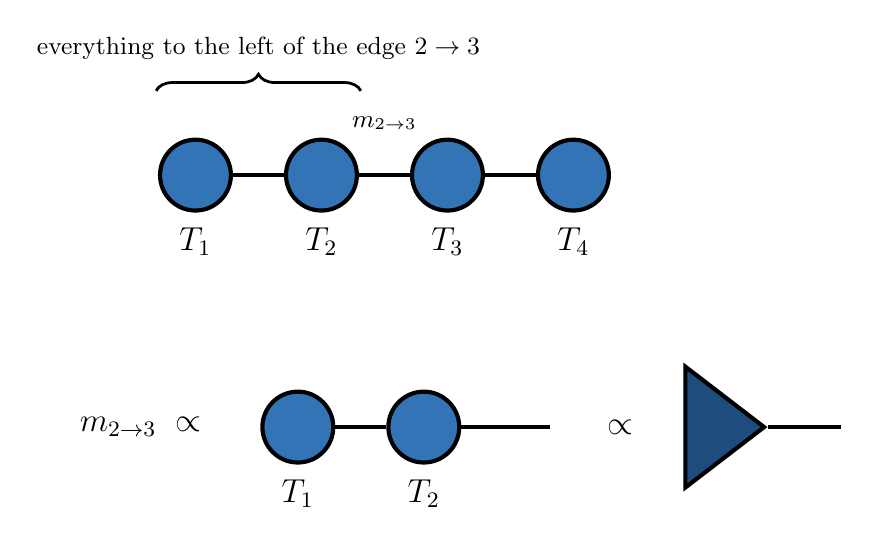
\begin{tikzpicture}
  % the network on a path graph
  \foreach \i in {1,...,4} { \node[tensor] (t\i) at (1.6*\i,0) {}; \node[lab] at (1.6*\i,-0.85) {$T_\i$}; }
  \foreach \i/\j in {1/2,2/3,3/4} { \draw[leg] (t\i) -- (t\j); }
  \node[lab,anchor=south] at (1.6*2.5,0.45) {\small$m_{2\to3}$};
  \draw[decorate,decoration={brace,amplitude=6pt,raise=2pt},line width=1pt] (1.1,1.0) -- (3.7,1.0);
  \node[anchor=south] at (2.4,1.35) {\small everything to the left of the edge $2 \to 3$};
  % the message
  \begin{scope}[yshift=-3.2cm]
    \node[lab] at (0.9,0) {$m_{2 \to 3} \;\propto$};
    \node[tensor] (a) at (2.9,0) {}; \node[lab] at (2.9,-0.85) {$T_1$};
    \node[tensor] (b) at (4.5,0) {}; \node[lab] at (4.5,-0.85) {$T_2$};
    \draw[leg] (a) -- (b);
    \draw[leg] (b) -- ++(1.6,0);
    \node[lab] at (7.0,0) {$\propto$};
    \node[msg] (M) at (8.2,0) {};
    \draw[leg] (M) -- ++(1.6,0);
  \end{scope}
\end{tikzpicture}
\end{document}
